\documentclass[a4paper,11pt]{article}
\usepackage[utf8]{inputenc}
\usepackage[ngerman]{babel}
\usepackage{a4wide,url,graphicx}

\usepackage[labelfont=bf]{caption}
\captionsetup{labelfont = sc, textfont = it}

\title{Praktikumsbericht zur Entwicklung\\ einer Mess-Station zur
  Luftqualitätsbestimmung} 
\author{Martin George}
\date{10.2019 -- 06.2020}

\parindent0pt
\parskip3pt

\begin{document}
\maketitle
\begin{abstract}
  Der Bericht stellt die Ergebnisse meiner Beschäftigung am Institut für
  angewandte Informatik (Infai) im Zeitraum vom 01.10.2019 bis zum 30.06.2020
  vor.
\end{abstract}
\tableofcontents
\newpage

\section{Einleitung}
Im Oktober 2019 habe ich die Stelle am Institut für angewandte Informatik (im
Folgenden \textit{Infai}) in der Forschungsgruppe um Dr. Michael Martin und
Norman Radtke angetreten, mit dem Ziel, die Arbeit an der Entwicklung eines
Prototyps für die Messung von Umweltdaten fortzuführen, die ein Praktikant vor
mir begonnen hatte.

Das allgemeine Ziel des Vorhabens war es, eine Mess-Station zu entwickeln, die
in der Lage ist, verlässlich bestimmte Parameter zur Bewertung von
Luftqualität zu erheben, dabei jedoch günstig in der Fertigung ist. Letzteres
sollte durch Verwendung preiswerter Sensoren erreicht werden. Eine weitere
wichtige Rolle spielte der Fokus auf der LoRa-Technologie zur Übertragung der
Messdaten von der Mess-Station. In der Zeit vor meinem Praktikumbeginn wurden
deshalb schon einige Hardware-Komponenten getestet, miteinander verglichen und
schließlich ein erster Prototyp angefertigt, bei dem eine Reihe von Sensoren
verbaut war. Auf die genaue Konfiguration dieses ersten Prototyps, von dem
ausgehend ich weitere Prototypen entwickelt habe, gehe im Folgenden noch
weiter ein.

Das Projekt war zu Beginn noch in einer Kooperation mit der Stadt Halle
eingebettet, die das Ziel verfolgte, durch den Einsatz von verteilten Sensoren
zur Messung der Luftqualität eine evidenzbasierte Unterstützung einer
umweltsensitiven Stadtplanung und Verkehrssteuerung im Stadtgebiet Halle zu
entwickeln. Die Motivation war es also, ein System zum Monitoring der
Luftqualität zu entwickeln, vor allem hinsichtlich der hohen
Feinstaubbelastung, vornehmlich ausgelöst durch hohes Verkehrsaufkommen im
Straßenverkehr. Die Verwendung von breit verfügbaren Sensoren und
Microcontrollern aus dem DIY-Bereicht schien dabei ein valider Ansatz, um die
Kosten für solch ein Unterfangen niedrig zu halten. Die Kooperation kam nicht
zu Stande und spielte somit für die Zeit meiner Beschäftigung keine große
Rolle, jedoch entwickelten wir nichts desto weniger die Idee und die ersten
Prototypen unter der unveränderten Prämisse der möglichst geringen Baukosten
weiter, mit dem Ziel ein System zu entwerfen, das ein günstiges, flexibles und
valides Monitoring der Luftqualität, aber auch anderer Umweltdaten, im
städtischen Raum ermöglicht.

Um diesem Ziel näher zu kommen, habe ich während meiner Tätigkeit das Vorhaben
in verschiedene Richtung weiterentwickelt. Nach der Anlaufzeit, die ich
benötigte, mich ausreichend in die vorhanden Strukturen, nämlich die
LoRa-Technologie und die verwendeten Dienste im Internet-of-Things, den
Software-Stack und vor allem die Programmierung des Prozessors mittels
MicroPython, einzuarbeiten, entwickelte ich diverse Prototypen einer
Mess-Station, implementierte neue Sensoren, verbesserte die Treiber bestehender
Sensoren, erweiterte die Firmware um präzisere Messroutinen und verfolgte den
Ansatz einer autarken (batteriebetriebenen) Mess-Station. Schließlich führte
ich noch eine Reihe von Tests zur Reichweitenbestimmung des LoRa-Netzwerkes im
Leipziger Stadtgebiet durch, um schließlich eine erste -- für den Außeneinsatz
geeignete -- Mess-Station zu entwerfen und zu bauen, die dann in der Nähe des
Leipziger Hauptbahnhofs angebracht wurde.

Im Folgenden möchte ich nun auf manche der eben genannten Tätigkeitsfelder
noch etwas genauer eingehen.

\section{Tätigkeitsbeschreibung}
\subsection{Einarbeitung und Beschreibung der Ausgangssituation}

Der prototypische Aufbau einer Mess-Seinheit, der zu Beginn meiner Tätigkeit
bereits einige Zeit im Inneneinsatz in Betrieb war, bestand aus drei Sensoren
(\textit{DHT22} zur Messung von Temperatur und Luftfeuchtigkeit,
\textit{SDS011} Feinstaubsensor, \textit{MiCS-6814} zur Messung verschiedener
Gaskonzentrationen in der Luft, etwa NO2 und CO), sowie aus einem
\textit{Lopy4}-Entwicklerboard der Firma Pycom, welches die Sensormodule per
I2C- bzw UART-Schnittstelle ausliest. Das Lopy4-Board basiert auf einem
ESP32-Prozessor, der mittels MicroPython programmiert werden kann. Außerdem
ist neben einem Wifi-Modul ebenfalls ein LoRa-Modul auf dem Lopy4 verbaut. Die
ausgelesenen Messwerte können somit über eine LoRa-Bibliothek verpackt und
verschickt werden. Zum Empfang der Daten stand ein Eigenbau-Gateway bereit,
basierend auf einem Raspberry-Pi, das die Daten empfängt und über eine
Ethernet-Schnittstelle an das The-Things-Network (im Folgenden \textit{TTN})
weiterleitet.

Softwareseitig war auf dem Board eine basale Firmware zum Auslesen der
Sensoren und Versenden der Messwerte implementiert. Hier musste ich mich vor
allem mit der Funktionsweise der Sensoren und dem Schaltungsaufbau
auseinandersetzen.

Für die Verarbeitung, persistente Speicherung und Visualierung der Daten war
bereits im Backend ein Software-Stack, bestehend aus verschiedenen
Werbservices implementiert. Die auf dem TTN empfangenen Daten werden mittels
eines \textit{MQTT-Consumers} -- Bestandteil des Server-Agents
\textit{Telegraf} -- in eine \textit{InfluxDB} übertragen. Die dort persistent
gespeicherten Daten können dann anschließend über das Webinterface von
\textit{Grafana} visualisiert werden. Die drei genutzten Services Telegraf,
InlfuxDB und Grafana liegen in einzelnen Docker-Containern, die wiederum auf
dem Infai-Server laufen und permanent die Messdaten verarbeiten (Für eine
grafische Veranschaulichung des Stacks siehe Abbildung \ref{stack}). Da ich
mit allen drei verwendeten Services noch keine Erfahrung hatte, verwendete ich
einige Zeit darauf, mich mit dem Stack vertraut zu machen. Ebenso investierte
ich einige Zeit, um das Erstellen von Images und das Handling von Containern
in der Docker-Laufzeitumgebung zu erlernen.

Die Programmierung des Lopy4-Boards erfolgt über Plugins für Code-Editoren,
etwa Visual-Studio-Code. Die Sprache MicroPython ist eine effiziente, dabei
schmale, Implemtierung von Python3, die für den Betrieb auf Mikro-Prozessoren
optimiert ist. Sie enthält einen Teil der Python3 Standard-Bibliotheken.  Die
Einarbeitung wurde unterstützt durch die recht gute Dokumentation auf dem
Projekt-Repository, ebenso durch die umfassende Dokumentation von
MicroPython, des Lopy4-Boards und der verwendeten Webservices, vor allem des
TTN.

\subsection{Entwicklung und Bau einer Outdoor-Mess-Station}

Nach der Zeit der Einarbeitung recherchierte ich zunächst viel zu
verschiedenen Sensoren und deren Funktionsweise und Verfügbarkeit. Auch hier
gab es von meinem Vorgänger bereits einige Informationen über Projekte, die
ein -- unserem Ansatz ähnliches -- Vorhaben verfolgten, aber auch
Informationen über kommerzielle Mess-Stationen, die bereits auf dem Markt
verfügbar waren. Ich verfolgte das Ziel, möglichst bald einen Prototyp einer
Mess-Stationen entworfen und gebaut zu haben, der -- mit neuen Sensoren
ausgestattet -- in den Außeneinsatz gebracht werden konnte. Glücklicherweise
waren wir in der Lage, eine Kooperation mit dem Landesamt für Umwelt,
Landwirtschaft und Geologie (LfULG) in Sachsen einzugehen, die es uns
ermöglichen sollte, unsere Prototypen an einer der offiziellen Mess-Stationen
in Leipzig anzubringen. Dies versprach den Vorteil, dass wir die
Messgenauigkeit der von uns verwendeten Sensoren sehr genau bestimmten
könnten, da wir die durch unsere Mess-Station generierten Daten jeder Zeit mit
den -- öffentlich verfügbaren -- Daten der Leipziger Mess-Station vergleichen
könnten.

Wir entschieden uns für Mess-Station Leipzig-Mitte in der Nähe des
Hauptbahnhofs. Um sicher zu gehen, dass die Entfernung zum Gateway am Infai am
Goerderlering nicht zu groß ist, um verlässlich die LoRa-Datenpakete zu
empfangen, entwickelte ich ein simples Testgerät, das neben einem Akku, etwas
Peripherie und einem Lopy4-Board auch ein GPS-Modul beinhaltete, so dass es
mir möglich war, einen Standort via LoRa zu senden. Im Nachgang konnte ich
dann sehen, von welchen Standorten aus die Daten vom Gateway noch empfangen
wurden (siehe Abbildung \ref{range_node}). Zum Testen begab ich mich mit dem
Gerät in Richtung Hauptbahnhof. Bei der nachträglichen Analyse stellte sich
heraus, dass die LoRa-Verbindung stark genug war, wenn auch die Daten zum
Großteil über ein anderes -- öffentliches -- TTN-Gateway in der Nähe empfangen
wurden (siehe Abbildung \ref{bewegungsprofil}).

Nach einiger Recherche stand die Hardware-Konfiguration der zu bauenden
Mess-Station fest auf Grund von Preis und vermeintlicher Verlässlichkeit
entschieden fiel die Entscheidung auf die Verwendung des
\textit{PMS7003}-Feinstaubsensors, des \textit{BME280}-Sensors, zur Messung
von Temperatur, Luftfeuchtigkeit und Luftdruck, sowie des \textit{MiCS-6814}
zur Erhebung der CO- bzw. NO2-Konzentration in der Luft. Außerdem sollte ein
\textit{Neo-6M}-GPS-Modul verbaut werden. Die Erprobung dessen Nutzen zielte
auf ein perspektivisches Szenario ab, in dem mehrere baugleiche Stationen im
Stadtgebiet verteilt werden und somit eine Ortung und Zuordnung der
Mess-Stationen unbedingt erforderlich wäre.

Ich entschied mich für einen redundanten Aufbau mit zwei Lopy4-Boards und
zweimal dem gleichen Sensoren-Set. Das sollte die Möglichkeit schaffen, auch
Sensoren untereinander vergleichen zu können, um so etwa festzustellen, ob
baugleiche Sensoren im selben Setting bereits Messunterschiede
aufzeigen. Außerdem sollte somit die Ausfallsicherheit erhöht werden. Diese
Maßnahme erwies sich auch als äußerst sinnvoll, da ich mich in den folgenden
Wochen gelegentlich zur Mess-Station begeben musste, um das System zu rebooten
und zu debuggen. Aus den Erfahrungen konnte ich dann Firmware-Upgrades
entwickeln und auf die Lopy-Boards spielen, die nachhaltig zu einer
Stabilisierung des System geführt haben. Durch die Redundanz ist es aber
dennoch gelungen, eine weitestgehend lückenlose Datenabdeckung seit Dezember
2019 zu erreichen (leider sorgt die manchmal schwankende LoRa-Konnektivität
auch für Paketverluste und auch das Server-Backend lief zu Beginn nicht immer
fehlerfrei).

Die Sensoren wurden also in einem speziellen Lamellenschirm verbaut, der
ausreichende Luftzirkulation und ausreichend Wetterschutz bietet. Der Rest der
elektronischen Komponenten fand in einem wasserdichten Gehäuse Platz. Für die
Anbringung der Bauteile im Gehäuse und Lamellenschirm war es nötig, spezielle
Befestigungsteile zu entwerfen und zu fertigen. Dies geschah mittels
CAD-Software und einem Lasercutter. Die Hauptplatine, die das Lopy4-Board,
sowie das GPS-Modul und weitere Peripherie beheimatet, wurde ebenfalls selbst
entworfen und verlötet. Schließlich konnte die gesamte Mess-Station
zusammengebaut und -- nach einer Reihe von Tests -- an der Mess-Station der
LfULG am Leipziger Hauptbahnhof angebracht werden (siehe Abbildung
\ref{node_v1} und \ref{leipig_mitte}).

\subsection{Weiterentwicklung der Firmware}

Im Vorfeld hatte ich bereits Treiber für die neu verwendeten Sensoren in die
bestehende Firmware eingebunden, zum Teil waren diese gut dokumentiert frei
verfügbar, bei manchen Sensormodulen musste ich jedoch entweder eigene Treiber
unter zu Hilfenahme des technischen Datenblatts des jeweiligen Sensors
schreiben, oder aber Bibliotheken aus anderen Sprachen in MicroPython
übersetzen -- welche in den meisten Fällen entweder \textit{C} oder
\textit{Python} waren.

Neben der Implementierung neuer Treiber wurde die Firmware dahingehend
angepasst, so dass Mess- und Sendeintervalle im Einklang mit der
\textit{LoRa-Fair-Use-Policy}\footnote{\url{https://www.thethingsnetwork.org/docs/lorawan/duty-cycle.html}}
stehen.

In den weiteren Iterationen der Firmware wurden diverse Maßnahmen eingebaut,
welche die Stabilität des Systems steigern sollten, wie
\textit{Error-Handling} und die Übermittlung von Fehlercodes von der
Mess-Station an das TTN.

Zudem konnte die Genauigkeit von Messungen bestimmter Parameter verbessert
werden, indem Messroutinen angepasst wurden und somit Werte über einen
bestimmten Zeitraum ausgelesen, gespeichert und als laufender Mittelwert in
einem bestimmten Intervall an das Gateway gesendet wurden.

Auch verwendete ich einige Zeit auf die Erweiterung der Bibliotheken, die für
die Codierung und Decodierung der Messwerte verwendet werden, um zu
ermöglichen, dass für die Felder der Payload der LoRa-Message klare Bezeichner
verwendet werden können. Das erleichterte uns die Integration der Messdaten in
die InfluxDB und die anschließende Visualisierung in Grafana deutlich, da von
nun an gemessene Parameter (wie \textit{Temperatur},
\textit{CO-Konzentration}, etc) mit klar bezeichnenden Namen in der Datenbank
auftauchten.

Die Visualisierung musste ebenfalls an die neue Mess-Station angepasst
werden. Dafür erstellten wir neue Dashboards im Webinterface von Grafana, die
es uns später auch ermöglichen sollten, die Messwerte unserer Mess-Stationen
direkt mit den offiziellen Daten vergleichen zu können (siehe Abbildung
\ref{grafana}).

\subsection{Recherche und Testreihe hinsichtlich einer autarken Mess-Station}

Nachdem die Entwicklung und der Bau der Outdoor-Mess-Station vorerst
abgeschlossen waren, widmete ich mich der Idee, die Hardwarekonfiguration, die
in dieser zum Einsatz gekommen war, um solche Komponenten zu erweitern, die
einen autarken Betrieb ermöglichen könnten. Das bisherige Design basierte auf
einem 5V-Schaltnetzteil, ein Vorhandensein eines 230V-Stromanschlusses war für
die Installation also zwingend nötig. Bei der Anbringung an der Mess-Station
Leipzig-Mitte des LfULG war diese Voraussetzung zwar gegeben, aber
hinsichtlich des Vorhabens eine flexible Lösung für das
Luftqualitäts-Monitoring im städtischen Gebiet zu schaffen, wo eine
Stromversorgung über Kabel nicht an jeder Ecke frei zugänglich ist, lag es
also nahe, die Stromversung der Mess-Station autark zu gestalten.

Zu diesem Zwecke recherchierte ich einige gängige Lösungen, die alle auf einem
Lipo-Akku und einem Solarpanel in Verbindung mit einem Lademodul
basierten. Ich stellte einige Berechnungen an, um herauszufinden, welchen
Energiebedarf die verwendeten Sensoren in Kombination mit dem Lopy4-Board in
Summe haben, wie hoch die Kapazität eines Akkus mindestens sein muss, um auch
an bewölkten Tagen den Betrieb der Mess-Station sicherstellen zu können und wie
groß das Solarpanel gewählt werden sollte, um eine möglichst effiziente
Wiederaufladung des Akkus gewährleisten zu können.

Wir bestellten einige Bauteile und ich konzeptionierte verschiedene
Testaufbauten, um neben den angestellten Rechnungen auch empirische Werte für
die gesuchten Parameter, wie Akkukapazität etc., generieren zu können. Zu
diesem Zweck entwarf und baute ich zwei simple Spannungssensoren, die sowohl
die Akkukapazität, als auch die Ladespannung des des Solarpanels messen
sollten. Die Daten, die meine Testreihen generierten, speiste ich wiederum
unter Zuhilfenahme des Server-Agents \textit{telegraf} in unsere InfluxDB ein,
um sie anschließend in Grafana visualieren zu können. Bei den Messungen zeigte
sich schnell, dass der Energiebedarf des gewählten Aufbaus sehr hoch ist,
sodass kein vernünftig dimensionierter Akku den Betrieb für längere Zeit hätte
sichern könnte. Für die Abweichung der empirischen Daten von den berechneten
waren hauptsächlich die -- zum Teil -- ungenauen Angaben zum Strombedarf der
Sensoren in den Datenblättern, aber auch der Overhead durch das von mir
verwendete Solar-Lademodul verantwortlich.

Ich fing somit an, die Firmware entsprechend anzupassen. Und zwar sollten
Messintervalle vergrößert werden und das Lopy-Board, sowie alle Sensoren,
zwischen den Messungen in einen \textit{deep-sleep}-Zustand gesendet werden.
Dieses Vorhaben erwies sich zwar als erfolgreich hinsichtlich des
Energieverbrauchs, war in der Praxis jedoch auf Grund des
Authentifizierungs-Protokolls des LoRa-Netzwerkes nicht ganz einfach
umsetzbar. Damit die LoRa-Verbindung trotz Minimalbetrieb des Mess-Station
nicht verloren ging, mussten die LoRa-Schlüssel im NVRAM des Lopy
zwischengespeichert und wieder ausgelesen werden.

Ein weiteres Problem war allerdings der hohe Energieverbrauch des Feinstaub-
und Gassensors, deren Lüfter, respektive Heizmodul, einen hohen Stromverbrauch
verursachten, jedoch für die valide Messung elementar waren. Letztendlich kam
ich zum Schluss, dass sich ein autarker Betrieb grundsätzlich mit besseren
Hardware-Komponenten zum Power-Management und einer adaptiven Messroutine, die
Messintervalle am Akkustand anpasst, vernünftig realisieren ließe.

\subsection{Dokumentation und Diverses}

Meine Tätigkeit dokumentierte ich hauptsächlich in dem dafür vorgesehenem
Projekt-Reposi\-tory auf dem Infai-internen GitLab. Neben der
Versionsverwaltung des Source-Codes der Firmware der Mess-Stationen nutzte ich
das Repository auch für die Dokumentation der Hardware-Konfiguration der von
mir gebauten Prototypen, der Ablage von Schaltplänen, die im Laufe der
Entwicklung der Prototypen erstellt wurden, technischen Zeichnung, 3D-Daten
bestimmter Bauteile, die ich angefertigt habe, sowie
Prozessbeschreibungen. Ebenso pflegte und erweiterte ich während meiner
Tätigkeit Recherchelisten zu verschiedenen Bereichen des Projekts, sei es zu
verfügbaren Sensoren, ähnlichen Projekten, kommerziellen Anbietern von
Mess-Stationen etc.

\section{Ausblick}
\label{section:ausblick}

Gegen Ende der Praktikumstätigkeit verlagerte sich der Projektfokus vorerst
weg vom Prototyping und eher hin zu einer vertiefenden Recherche hinsichtlich
weiterer messbarer Parameter wie Lärm, Co2 und Ozon. Auf Grund der mäßigen
Perfomance der Akku-Betriebenen Prototypen und vor dem Hintergrund des
Bestrebens, weitere Sensoren zu implementieren, die zum Teil einen hohen
Energieverbrauch während eines Messintervalls aufweisen, wurde die Arbeit an
einer autarken Lösung vorerst eingestellt und die Planung im Kontext von
Settings weitergeführt, die eine Spannungsversorgung am Ort der Anbringung
vorsehen (etwa durch Laternenmasten, Ampeln, etc.).

Ein weiterer Aspekt, der stärker in den Vordergrund trat, waren Überlegung
hinsichtlich einer Korrektur der von uns erhobenen Messwerte. Es zeigte sich
nämlich recht schnell, dass die von uns verbauten -- günstigen -- Sensoren, im
Vergleich zu den vom LfULG verwendeten Mess-Systemen, weitaus schlechtere Daten
lieferten. Da die Entwicklung der Mess-Stationen jedoch weiterhin unter der
Prämisse der günstigen Fertigung stand, das Verbauen teurerer -- vermeintlich
besserer -- Sensoren als Lösung für dieses Problem also nicht in Frag kam,
sollten Ansätze entwickelt werden, mit Algorithmen (etwa des maschinellen
Lernens) den Messfehler aus den übermittelten Werten der günstigen Sensoren im
Nachhinein korrigieren zu können.

\pagebreak
%\printbibliography[heading=bibintoc,title=Quellenverzeichnis]
\appendix
\section{Abbildungen}

In diesem Anhang befinden sich die im Text referenzierten Abbildungen. 

%Stack Übersicht
\bigskip\noindent
\begin{minipage}{\linewidth}
  \captionsetup{format=plain, labelfont=bf, font=small} \centering
  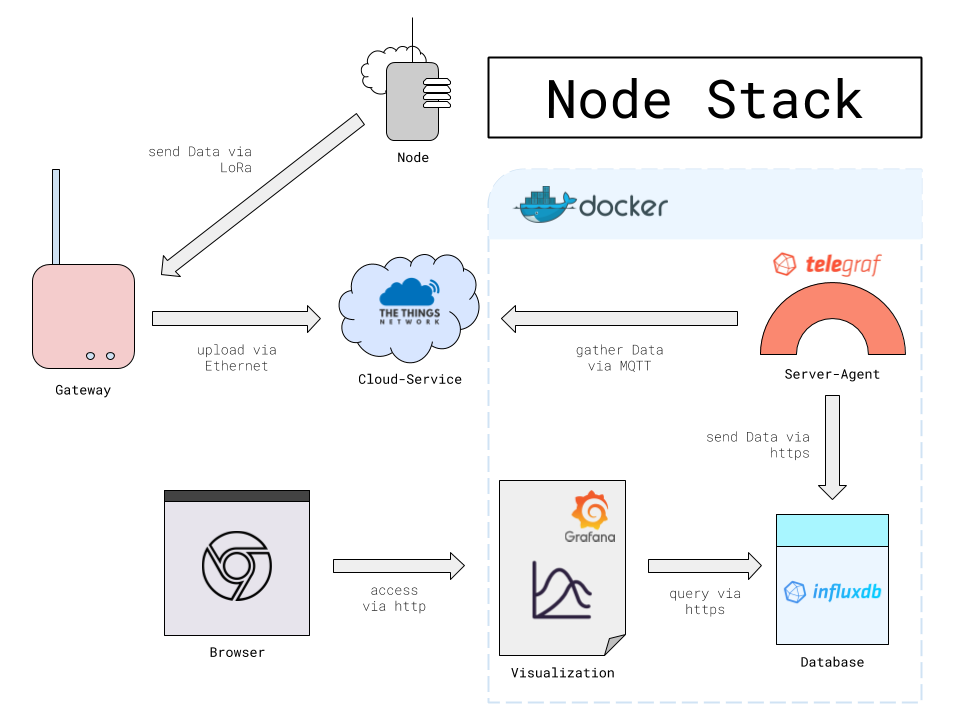
\includegraphics[width=\linewidth]{img/Node_Stack.png}
  \captionof{figure}{Datenfluss im Prototyp-Aufbau -- von der Mess-Station
    (Node) bis zur Visualisierung im Browser via
    \textit{Grafana} \label{stack}}
\end{minipage}

%Bild Range Node
\bigskip\noindent
\begin{minipage}{\linewidth}
  \captionsetup{format=plain, labelfont=bf, font=small}
  \centering
  %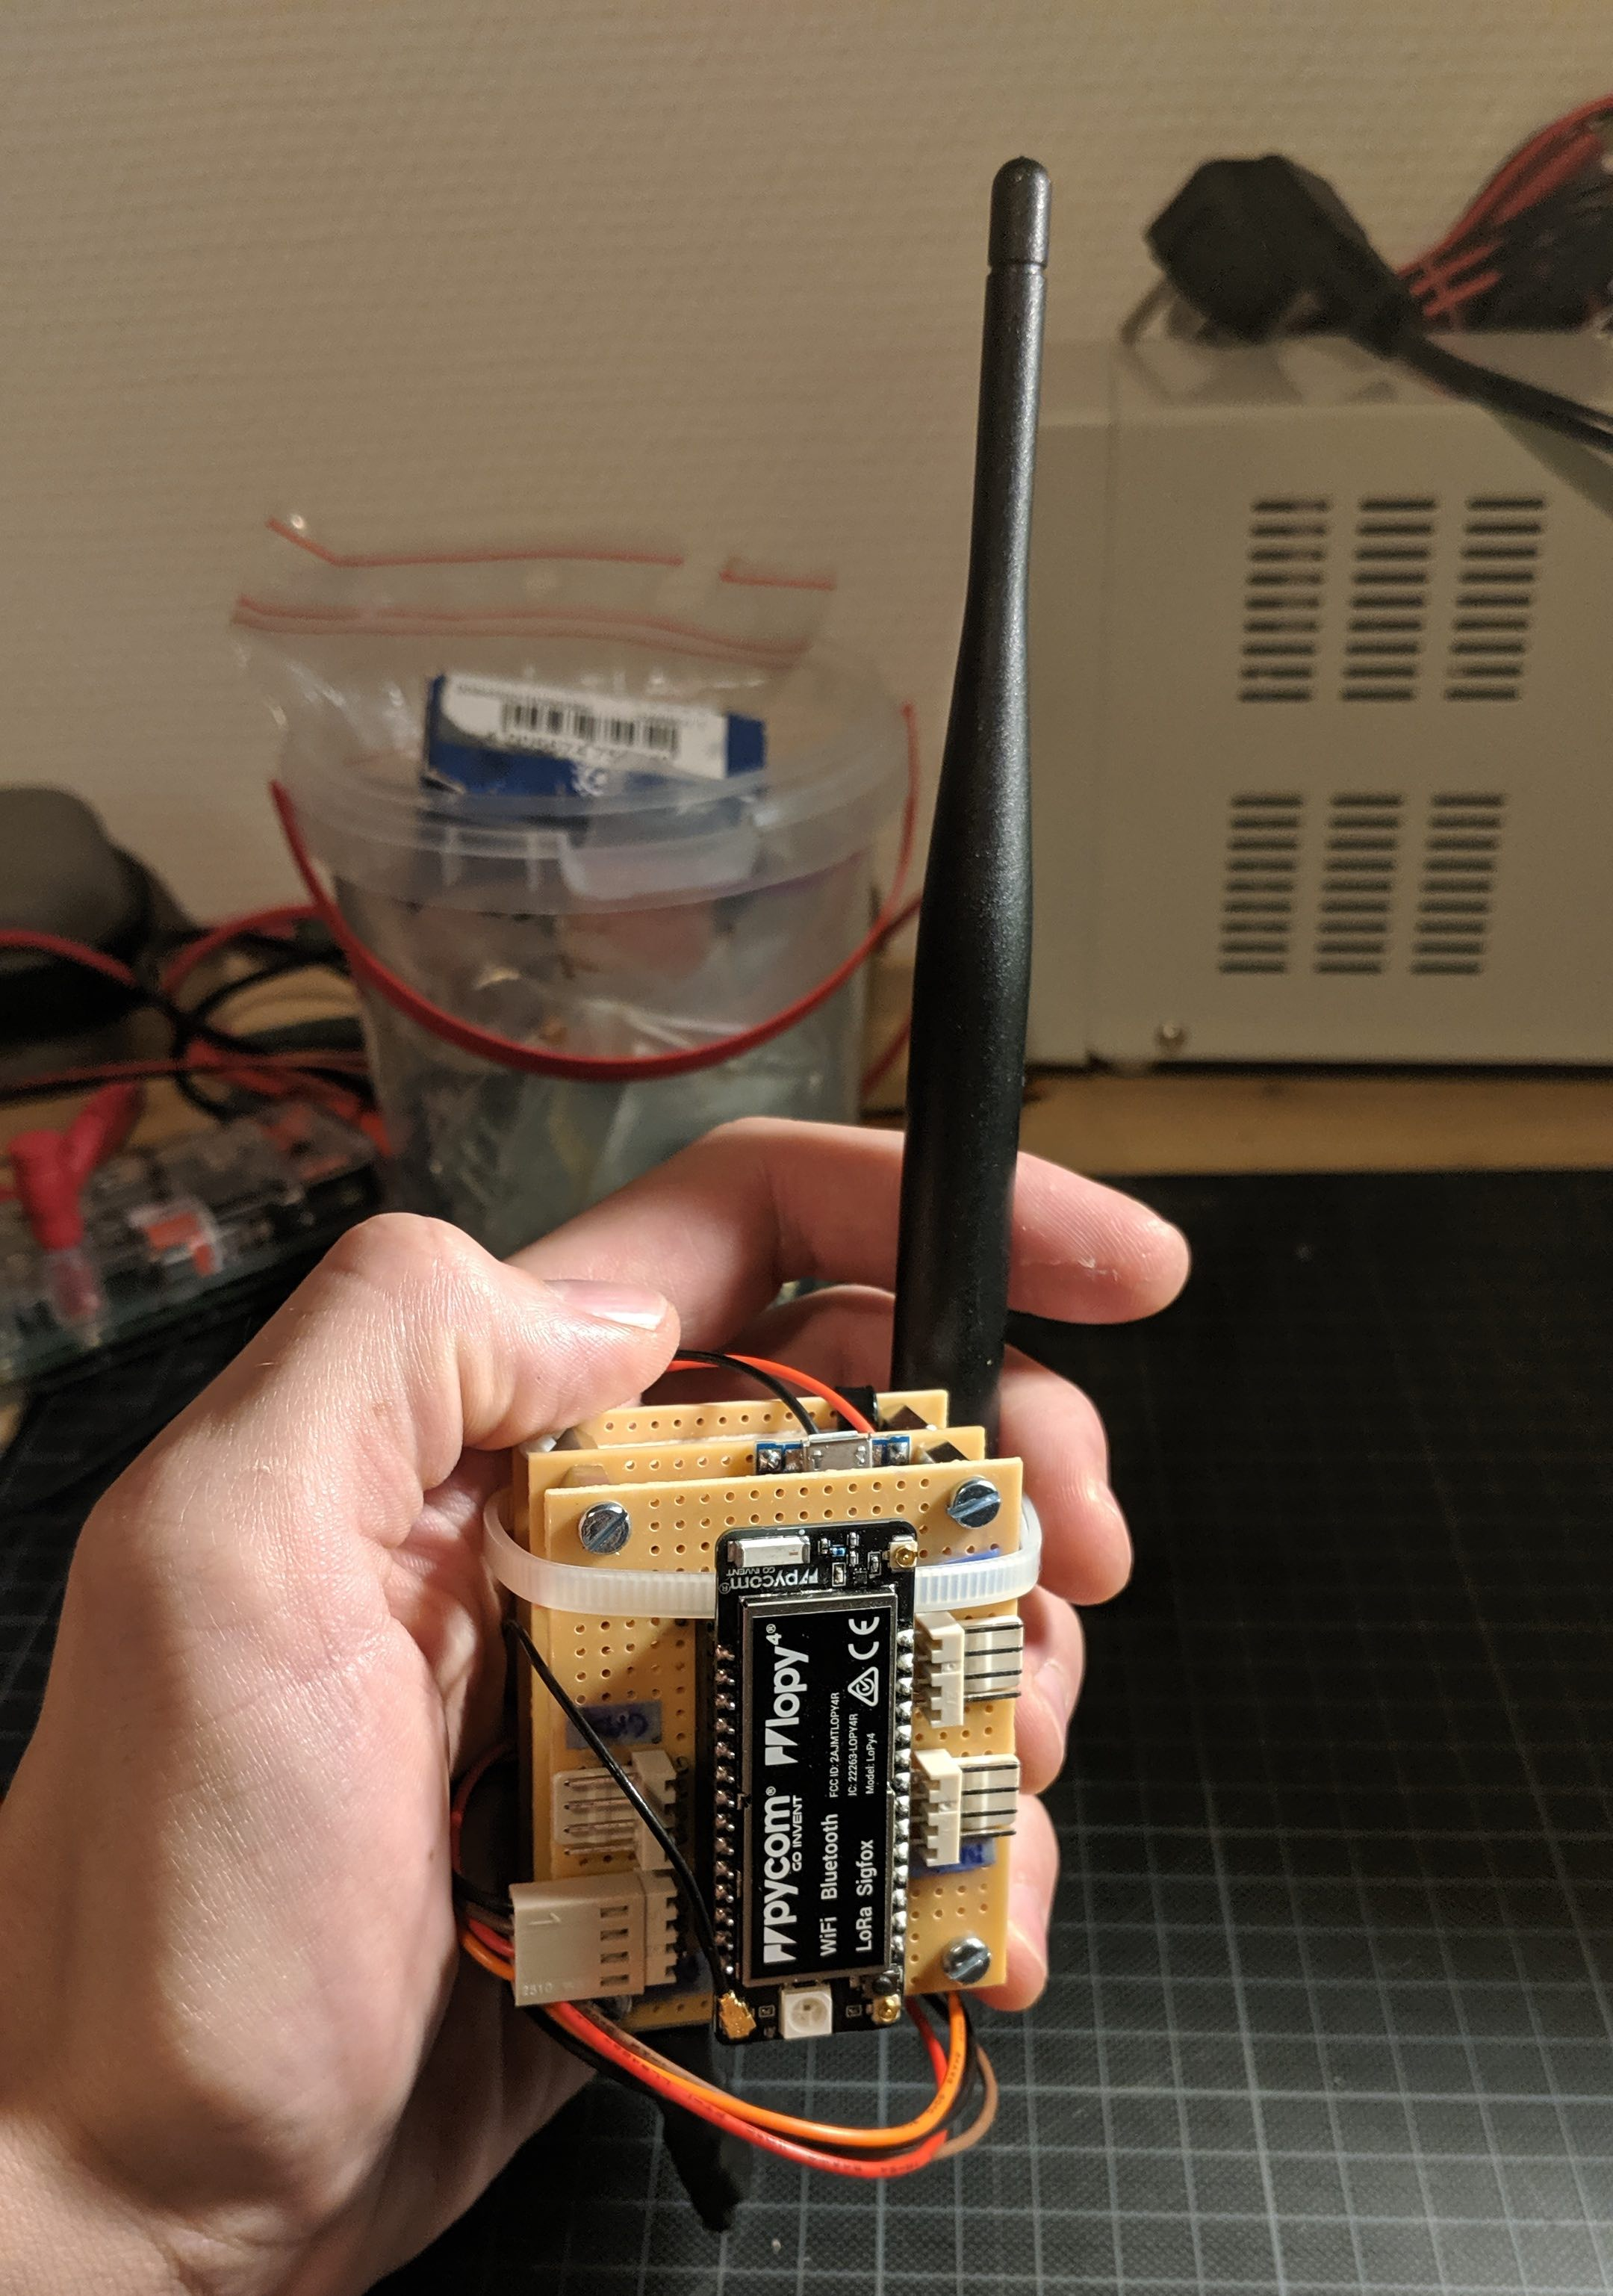
\includegraphics[width=\linewidth]{img/range_node.jpg}
  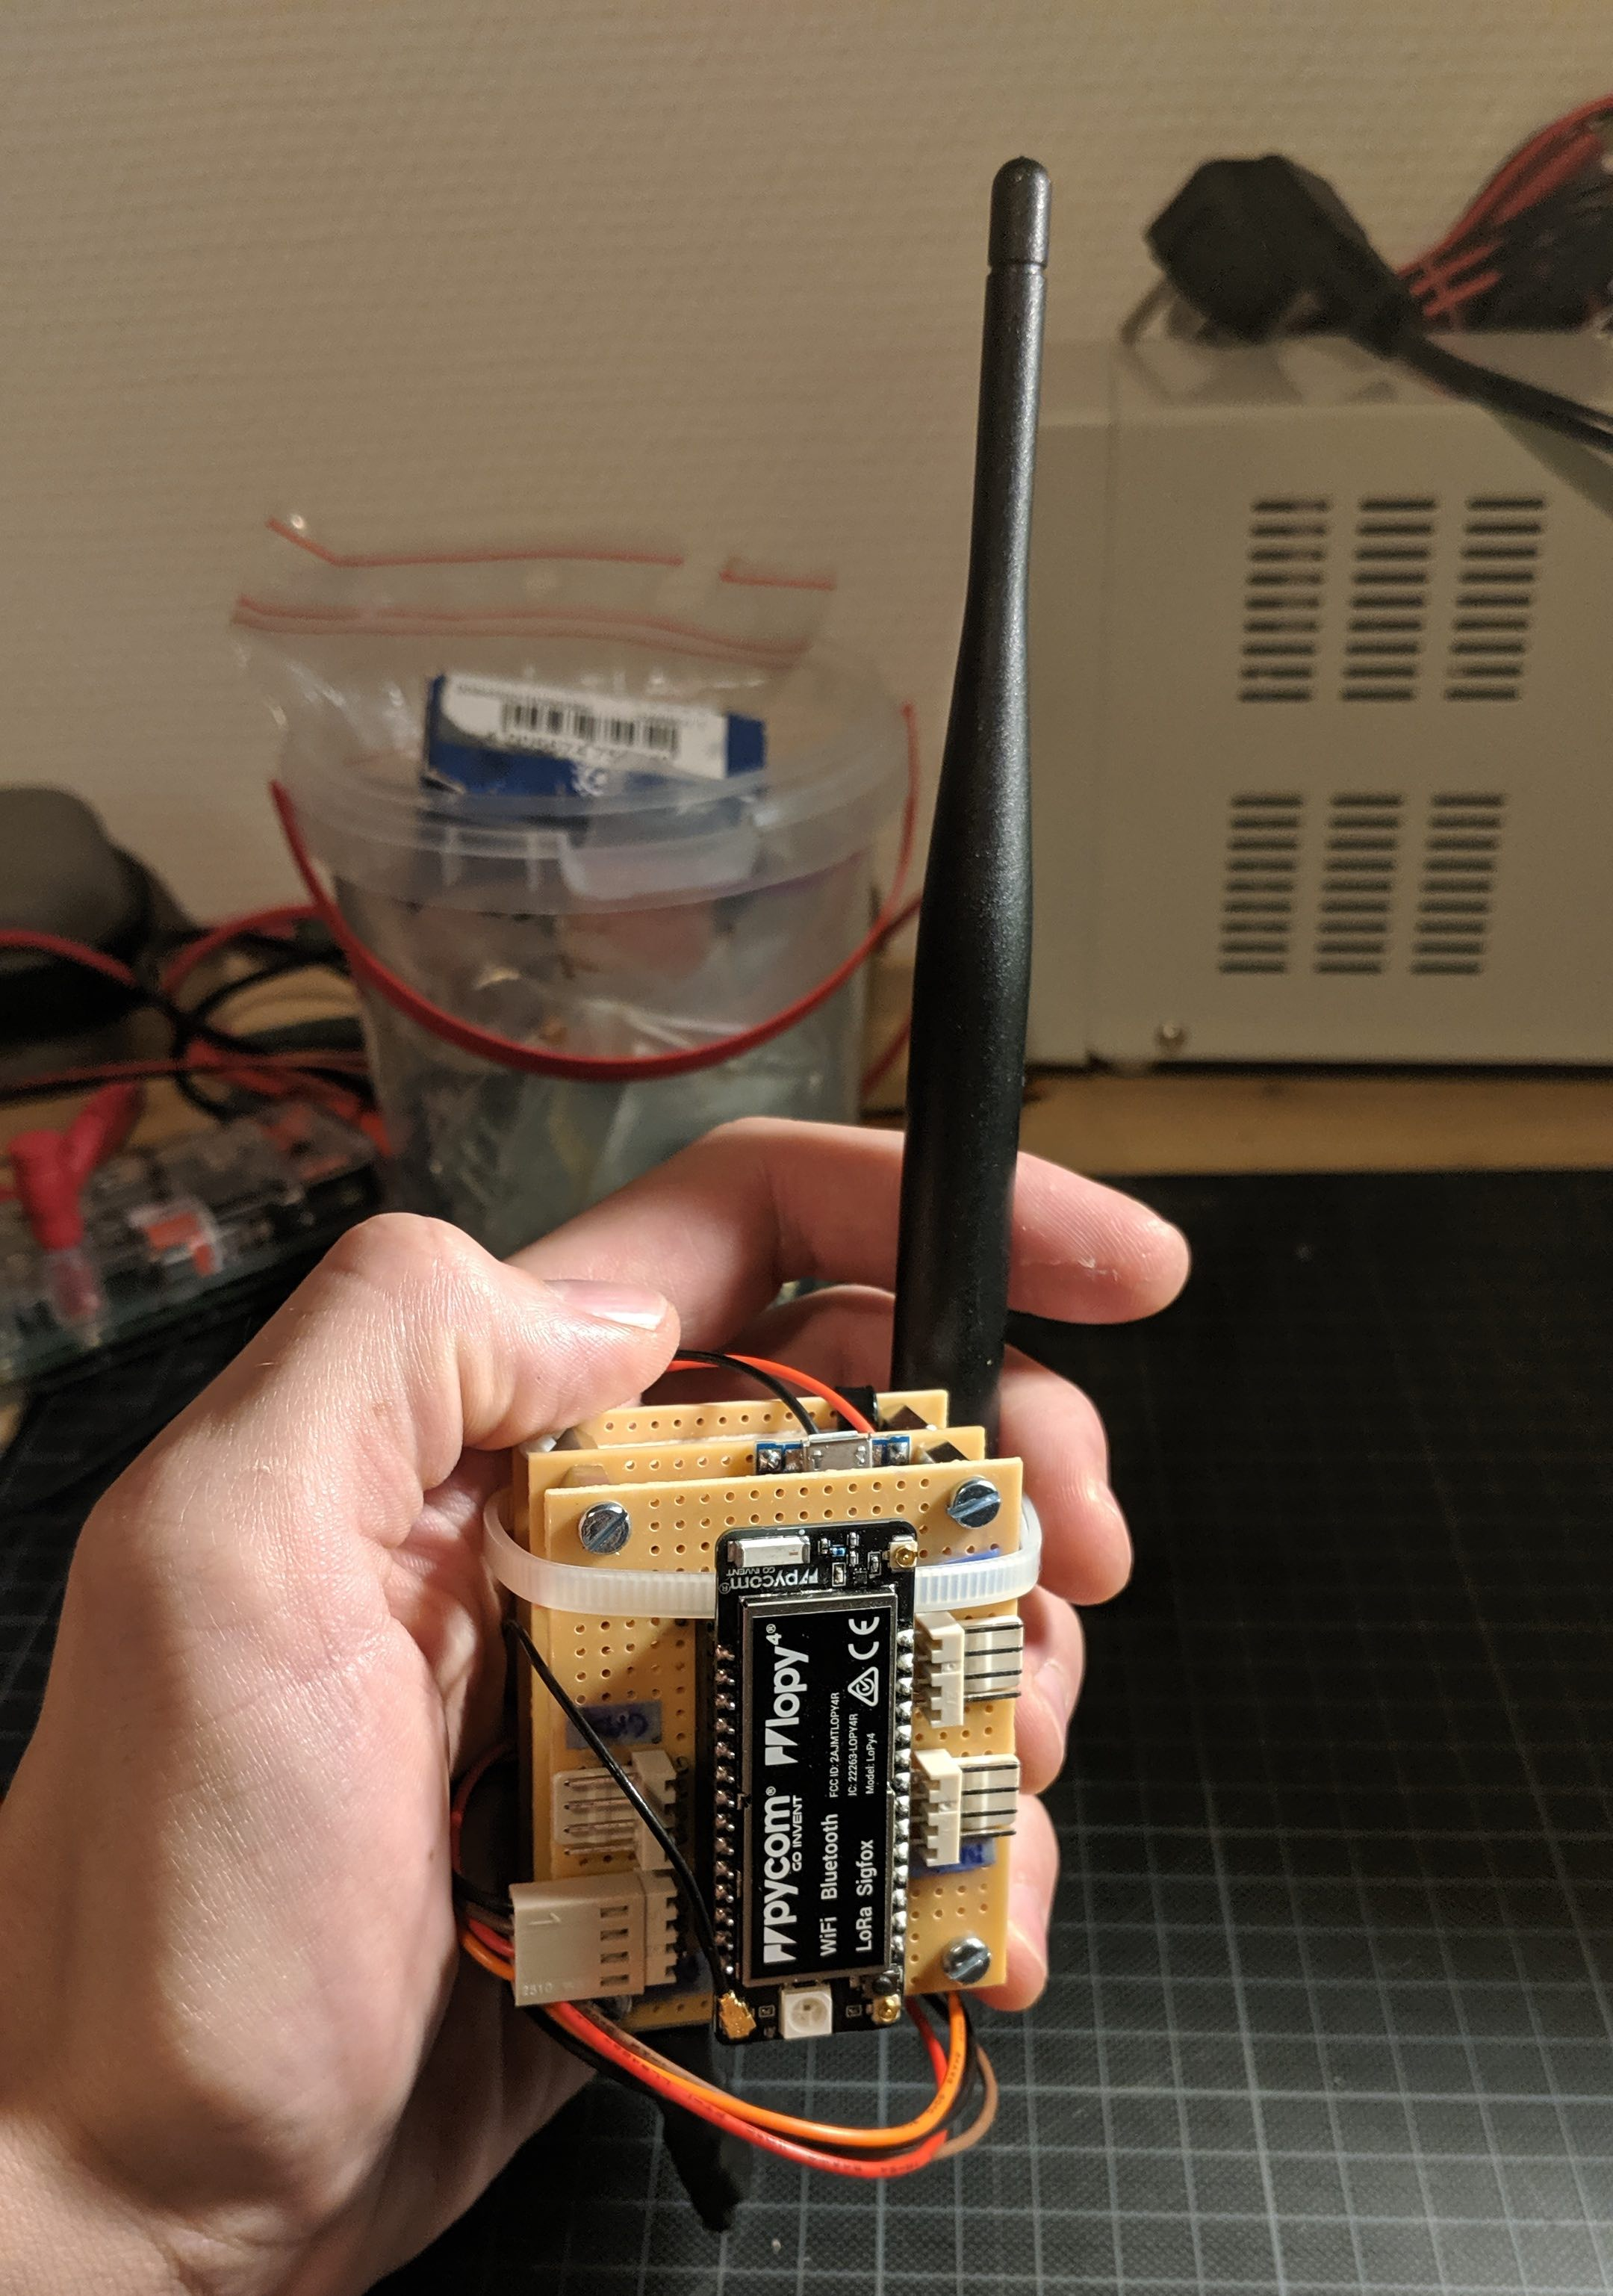
\includegraphics[width=6cm]{img/range_node.jpg}
  \captionof{figure}{Testaufbau bestehend aus einem Akku, einem Lopy4-Board,
    einer Lora-Antenne, eines GPS-Moduls und etwas Peripherie, zur Messung der
    Reichweite im LoRa-Netzwerk im Stadtgebiet \label{range_node}}
\end{minipage}

%Extra space between Abbildungen
\vspace{1cm}

%Bild Bewegungsprofil
\bigskip\noindent
\begin{minipage}{\linewidth}
  \captionsetup{format=plain, labelfont=bf, font=small}
  \centering
  %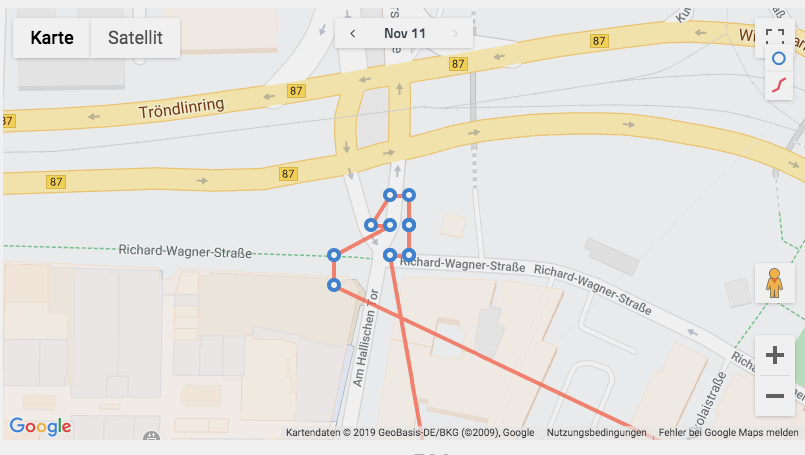
\includegraphics[width=15cm]{img/bewegunsprofil.png}
  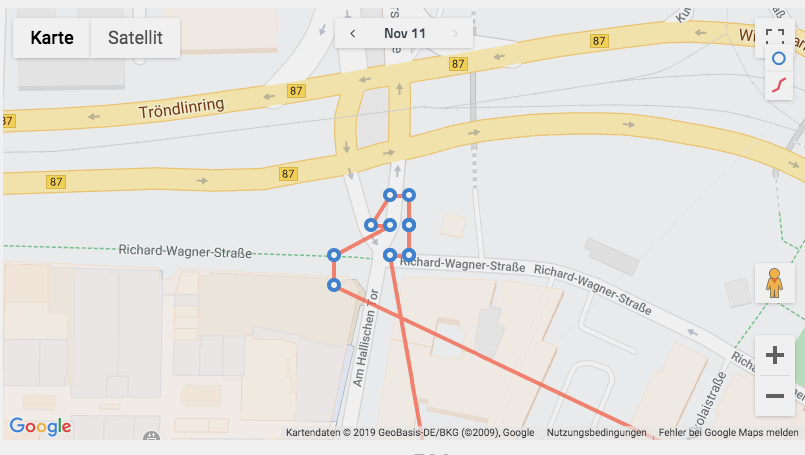
\includegraphics[width=\linewidth]{img/bewegunsprofil.png}
  \captionof{figure}{Auswertung der Standortdaten, die beim Testen der
    LoRa-Reichweite um die Mess-Station Leipzig-Mitte herum in der Nähe des
    Leipziger Hauptbahnhofs entstanden sind \label{bewegungsprofil}}
\end{minipage}

%Bild Node V1
\bigskip\noindent
\begin{minipage}{\linewidth}
  \captionsetup{format=plain, labelfont=bf, font=small}
  \centering
  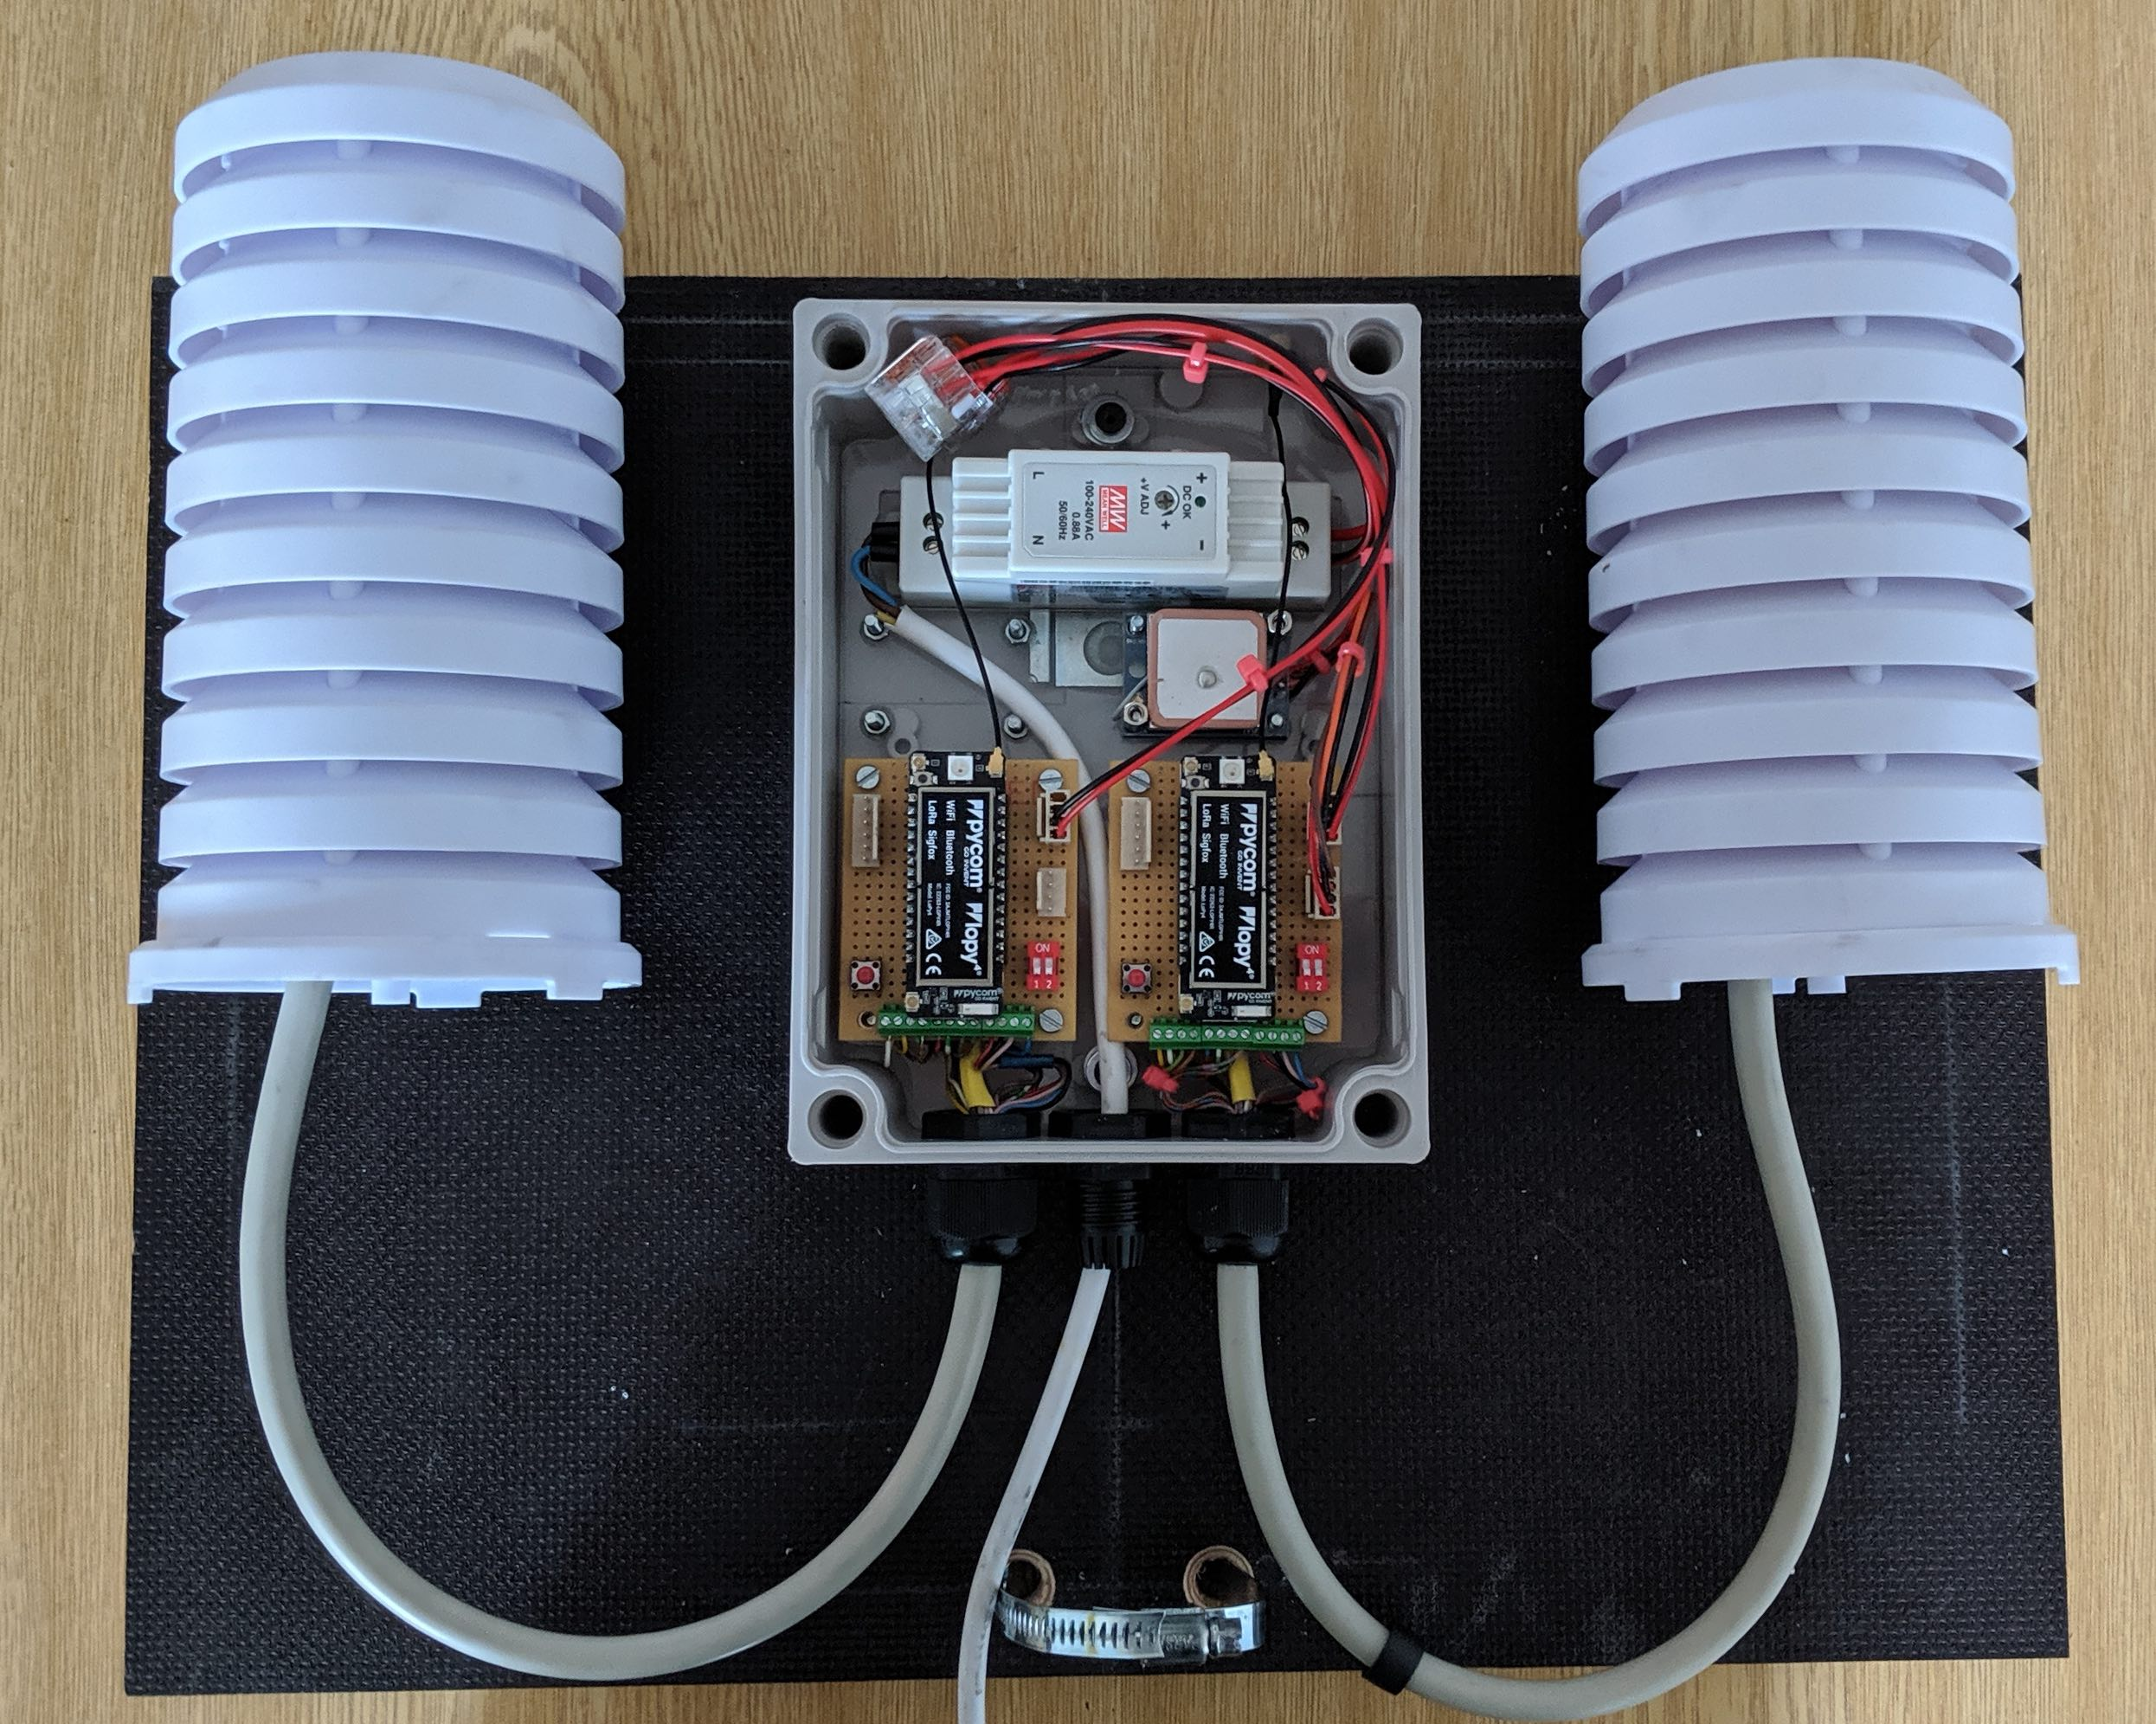
\includegraphics[width=\linewidth]{img/node_v1.jpg}
  \captionof{figure}{Der fertige Prototyp der ersten Outdoor-Mess-Station -- zu
    sehen ist der redundante Aufbau, die Lamellenschirme mit den Sensoren,
    sowie die Lopy4-Boards und Peripherie in einem wasserdichten
    Gehäuse. \label{node_v1}}
\end{minipage}

%Leipzig Mitte
\bigskip\noindent
\begin{minipage}{\linewidth}
  \captionsetup{format=plain, labelfont=bf, font=small}
  \centering
  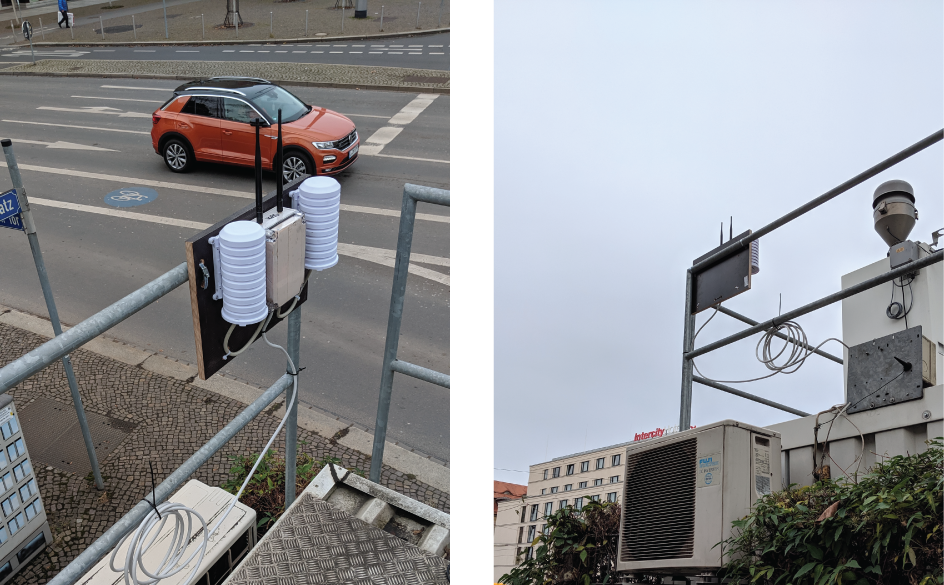
\includegraphics[width=\linewidth]{img/leipzig_mitte.png}
  \captionof{figure}{Bilder der Mess-Station nach Montage an der Station
    Leipzig-Mitte des sächsischen Landesamt für Umwelt, Landwirtschaft und
    Geologie (LfULG) \label{leipig_mitte}}
\end{minipage}

%Extra space between Abbildungen
\vspace{1cm}

%Grafana Dashbaord
\bigskip\noindent
\begin{minipage}{\linewidth}
  \captionsetup{format=plain, labelfont=bf, font=small}
  \centering
  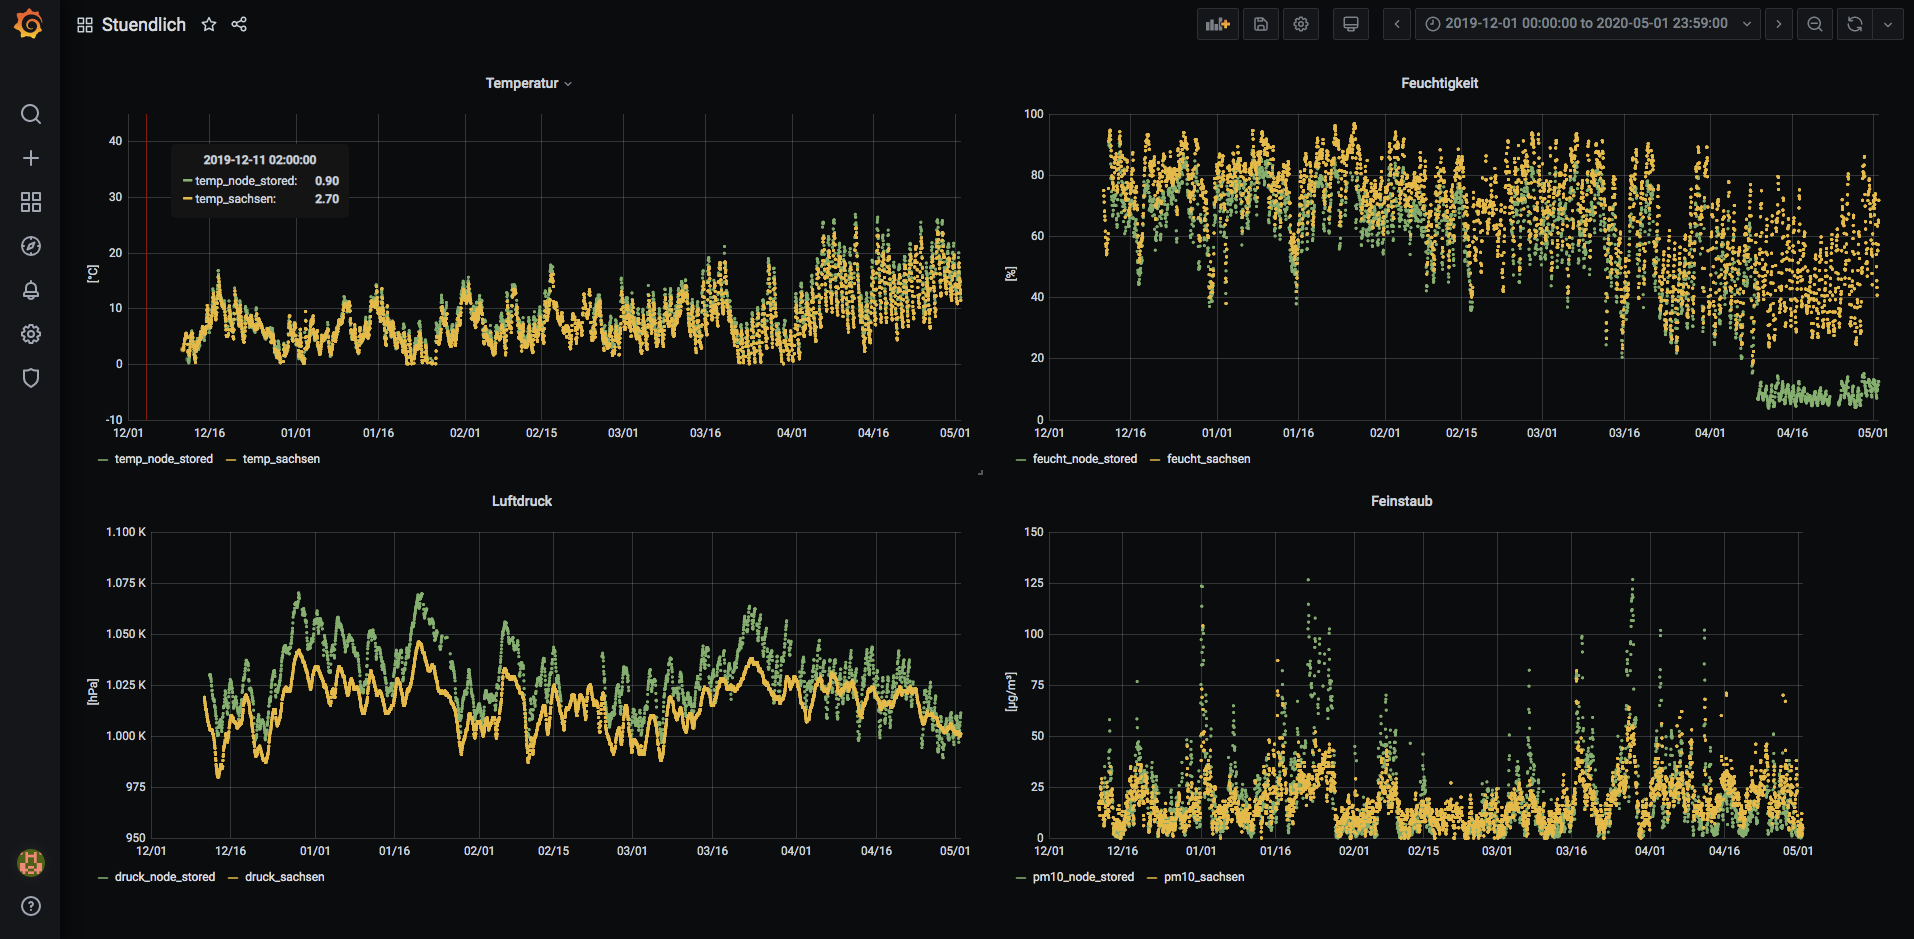
\includegraphics[width=\linewidth]{img/grafana.png}
  \captionof{figure}{Screenshot des Grafana-Interface -- Messpunkte des
    Prototyps im Vergleich zu den Messwerten der offiziellen Mess-Station
    Leipzig-Mitte im Zeitraum Dezember 2019 bis einschließlich Mai
    2020 \label{grafana}}
\end{minipage}

\end{document}

